\documentclass[mathserif]{beamer}

\usepackage{parskip}
\usepackage{amsmath}
\usepackage{amssymb}
\usepackage{graphicx}

\frenchspacing

\logo{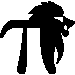
\includegraphics[width=0.075\textwidth]{../Logo}}

\usetheme{Rochester}
\usecolortheme{whale}
%\beamertemplatenavigationsymbolsempty

\AtBeginSection[] {%
	\begin{frame}
		\frametitle{Table of Contents}
		\tableofcontents[currentsection]
	\end{frame}
}

\newenvironment{compactmath}[1][\normalsize]%
	{\begin{minipage}{\textwidth}\vspace{-0.75\baselineskip}#1\begin{equation*}}
	{\end{equation*}\end{minipage}}

\newenvironment{namedframe}[1]%
	{\begin{frame}\frametitle{#1}\framesubtitle{\secname}}
	{\end{frame}}


\usepackage{tikz}
\usepackage{xfrac}

\title{Sequences and Series}
\subtitle{Your soon-to-be new best friend $\heartsuit$}
\author{Samantha Unger}
\date{
\includegraphics{../LicenseLogo}\\\copyright{} Samantha Unger, 2017}

\begin{document}
	\frame{\titlepage}
	\section{Summations}
	\begin{namedframe}{Introduction to Sigma notation}
		What is Sigma notation?
		\begin{itemize}[<+(1)->]
			\item Fun, easy-to-use way to sum things up!
			\item Super similar to a counted loop in computer programming
		\end{itemize}
		\pause
		Fun fact: Sigma is the 18th letter of the Greek alphabet, and is transliterated as ``s''.
	\end{namedframe}
	\begin{namedframe}{Using Sigma notation}
		\begin{compactmath}[\Large]
			\sum_{n=1}^{4}n
		\end{compactmath}
		The Sigma notation consists of several components. In the example above, we have:
		\begin{description}
			\item[$n$ under Sigma] Index of summation. Some people use $i$, $k$, or $x$
			\item[$1$] First value of $n$ (can be anything)
			\item[$4$] Term we end on
			\item[$n$ after Sigma] Formula for each turn
		\end{description}
		\sep
		\[\sum_{n=1}^{4}n = 1 + 2 + 3 + 4 = 10\]
	\end{namedframe}
	\begin{namedframe}{Example}
		Let's try some quick maths!

		We'll do this one together.

		There's more on your worksheet.
	\end{namedframe}
	\begin{namedframe}{Some \emph{super-cool} and \emph{super-useful} properties}
		Let's talk about why these work:

		\sep

		Multiplying by a constant:
		\[\sum_{k=m}^{n}ca_k = c\sum_{k=m}^{n}a_k\]

		\sep

		Adding/subtracting:
		\[\sum_{k=m}^{n}(a_k + b_k) = \sum_{k=m}^{n}a_k + \sum_{k=m}^{n}b_k\]
	\end{namedframe}
	\begin{namedbreakframe}{Summation shortcuts ;)}
		\begin{block}{Summing $1$ equals $n$}
			\[\sum_{k=1}^{n}1 = n\]
		\end{block}
		\begin{block}{Summing the constant $c$ equals $c \times n$}
			\[\sum_{k=1}^{n}c = nc\]
		\end{block}
		\framebreak
		\begin{alertblock}{A shortcut when summing $k$ (we will develop this later)}
			\[\sum_{k=1}^{n}k = \frac{n(n+1)}{2}\]
		\end{alertblock}
		\framebreak
		These ones are pretty cool and useful:
		\begin{block}{A shortcut when summing $k^2$}
			\[\sum_{k=1}^{n}k^2 = \frac{n(n+1)(2n+1)}{6}\]
		\end{block}
		\begin{block}{A shortcut when summing $k^3$}
			\[\sum_{k=1}^{n}k^3 = \left(\frac{n(n+1)}{2}\right)^2\]
		\end{block}
	\end{namedbreakframe}
	\begin{namedframe}{Try this!}
		\Huge
		Try the super cool practice word problem on your sheet!
	\end{namedframe}
	\section{Arithmetic Sequences}
	\begin{namedframe}{What is an arithmetic sequence?}
		\begin{itemize}
			\item A sequence of numbers where there is a constant difference between successive terms
			\item Example: $3,5,7,9,11$
		\end{itemize}
		\pause
		We can define the $n\textsuperscript{th}$ term with either of the following formulas:
		\[a_n = a_1 + (n-1)d \qquad a_n = a_m + (n-m)d\]
		Where we have:
		\begin{description}
			\item[$a_n$] the $n\textsuperscript{th}$ term
			\item[$n$] the term number
			\item[$d$] the constant difference
			\item[$m$] the $m\textsuperscript{th}$ term.
			\item[$a_1$] the first term of the series if we start counting from 1
		\end{description}
	\end{namedframe}
	\begin{namedframe}{Sum of finite arithmetic series}
		How can we easily sum a finite arithmetic series?
		\begin{itemize}[<+(1)->]
			\item Let me tell you about my main man Gauss\dots\footnote{This story may or may not be true,\\but I choose to believe it anyway.}
			\item Pair up your values and divide by 2!
		\end{itemize}
		\pause
		\begin{equation*}
			\begin{array}{lrrrrrrrrrrrrrrrrrrrrr}
				&    &1 &+  &2  &+  &3 &+  \dots &+ &98  &+ &99  &+ &100\\
				&+ &100 &+ &99  &+ &98 &+  \dots &+  &3  &+  &2  &+ &1\\\hline
				&  &101 &+ &101 &+ &101 &+ \dots &+ &101 &+ &101 &+ &101
			\end{array}
		\end{equation*}
		This is $101 \times 100$, which we know is $10100$.

		But we added up the numbers twice, so we need to divide by 2.
		\[10100 \div 2 = 5050 \qquad\qquad \text{\LARGE$\therefore$}\sum_{n=1}^{100}n = 5050\]
		\[S_n = \frac{n}{2}(a_1 + a_n)\]
	\end{namedframe}
	\section{Geometric Sequences}
	\begin{namedframe}{What is a geometric sequence?}
		\begin{itemize}
			\item Follows a pattern where each term in found by multiplying the previous term by a constant called the common ratio
			\item Examples: $3,6,12,24,48$ \hspace{2em} or \hspace{2em} $\frac{1}{2},\frac{1}{4},\frac{1}{8},\frac{1}{16}$
		\end{itemize}
		\pause
		We can define the $n\textsuperscript{th}$ term with any of the following formulas:
		\[a_n = a_{n-1} \times r \qquad a_n = a_1 \times r^{n-1}\]
		Where we have:
		\begin{description}
			\item[$a_n$] the $n\textsuperscript{th}$ term
			\item[$a_{n-1}$] the $(n-1)\textsuperscript{th}$ (previous) term
			\item[$a_1$] the first term of the series
			\item[$n$] the term number
			\item[$r$] the common ratio
		\end{description}
	\end{namedframe}
	\begin{namedframe}{Sum of finite geometric series}
		\begin{equation*}
			\begin{array}{lrrrrrrrrrrrrr}
				S_n  &= &a &+ &ar &+ &ar^2 &+ &ar^3 &+ \dots &+ &ar^{n-1} &  &    \\
				rS_n &= &  &+ &ar &+ &ar^2 &+ &ar^3 &+ \dots &+ &ar^{n-1} &+ &ar^n
			\end{array}
		\end{equation*}
		\begin{align*}
			S_n - rS_n &= a - ar^n\\
			S_n(1 - r) &= a(1-r^n)\\
			\therefore S_n &= a\left(\frac{1-r^n}{1-r}\right)
		\end{align*}
	\end{namedframe}
	\section{The Mind-blowing Part}
	\begin{namedframe}{What if\dots}
		What if I told you that the sum of some \emph{infinite} series wasn't infinite?

		\sep

		What if I told you that we can solve this? Can you sense the excitement?

		\begin{sizedmath}{\Huge}
			\sum_{k=1}^{\infty} 3\left(\frac{1}{2}\right)^{k-1}
		\end{sizedmath}
	\end{namedframe}
	\begin{namedframe}{Let's try one\dots}
		\[\sum_{n=1}^{\infty} \frac{1}{2^n} = \frac{1}{2} + \frac{1}{4} + \frac{1}{8} + \frac{1}{16} + \dots\]
		\pause
		Here are two ways to visualize this:
		\begin{columns}
			\begin{column}{0.5\textwidth}
				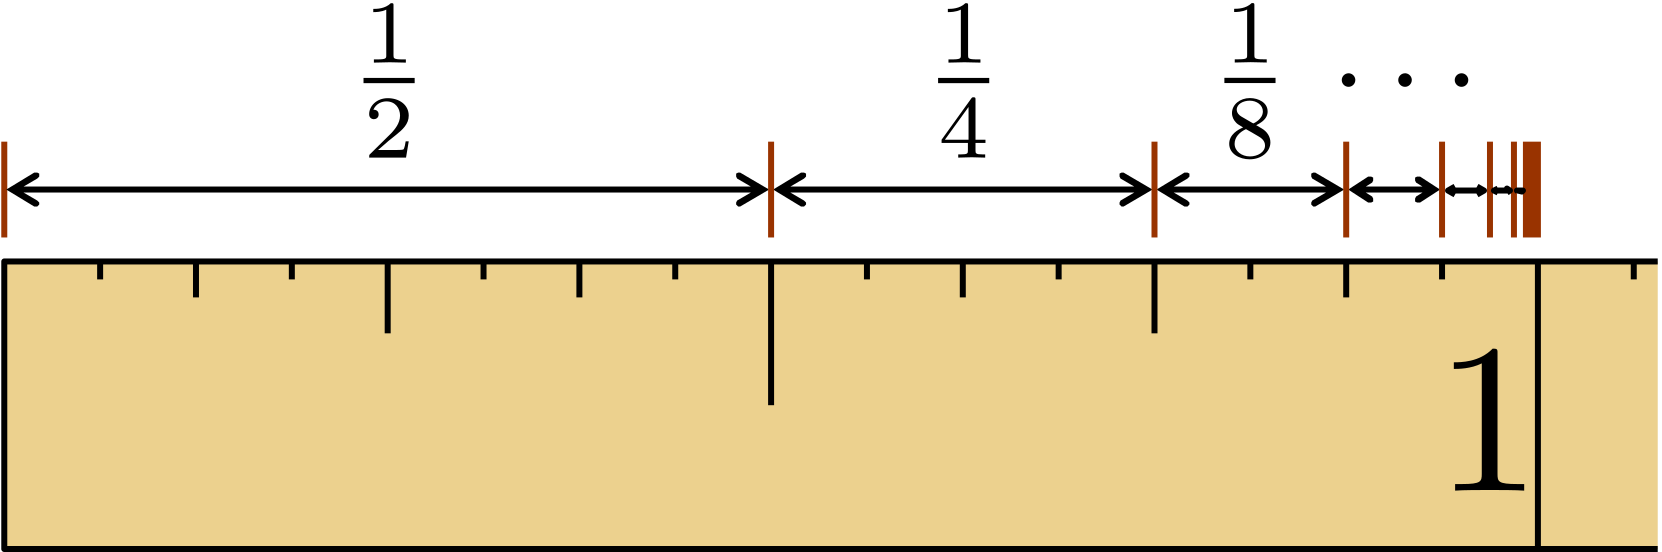
\includegraphics[width=\textwidth]{GeometricSegment}
			\end{column}
			\begin{column}{0.5\textwidth}
				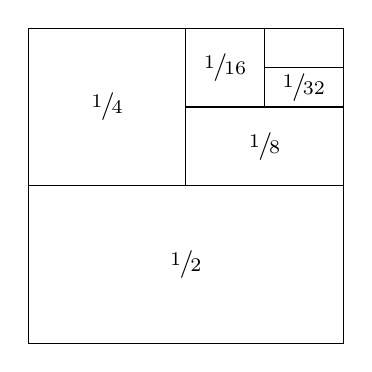
\begin{tikzpicture}
					\draw (0,0) rectangle (4,4);
					\draw (0,0) rectangle (4,2);
					\draw (0,2) rectangle (2,4);
					\draw (2,2) rectangle (4,3);
					\draw (2,3) rectangle (3,4);
					\draw (3,3) rectangle (4,3.5);

					\node at (2,1) {$\sfrac{1}{2}$};
					\node at (1,3) {$\sfrac{1}{4}$};
					\node at (3,2.5) {$\sfrac{1}{8}$};
					\node at (2.5,3.5) {$\sfrac{1}{16}$};
					\node at (3.5,3.25) {$\sfrac{1}{32}$};
				\end{tikzpicture}
			\end{column}
		\end{columns}
	\end{namedframe}
	\begin{namedframe}{What does that sum approach?}
		From the previous visualizations it's clear that:
		\[\sum_{n=1}^{\infty} \frac{1}{2^n} = \frac{1}{2} + \frac{1}{4} + \frac{1}{8} + \frac{1}{16} + \dots = 1\]
		Can we prove this with algebra?

		\sep

		\emph{Yes!}
	\end{namedframe}
	\begin{namedframe}{Solving algebraically}
		\begin{proof}
			We will call the whole sum $S$: $S = \frac{1}{2} + \frac{1}{4} + \frac{1}{8} + \frac{1}{16} + \dots$
			\pause

			Next, divide $S$ by $2$: $\frac{S}{2} = \frac{1}{4} + \frac{1}{8} + \frac{1}{16} + \frac{1}{32} + \dots$

			\sep

			Now, \emph{subtract} them!

			All the terms from $\frac{1}{4}$ onwards cancel out.

			\sep
			
			And we get: $S - \frac{S}{2} = \frac{1}{2}$.

			\sep

			Simplify: $\frac{S}{2} = \frac{1}{2}$.

			\sep

			So: $S = 1$.
		\end{proof}
	\end{namedframe}
	\begin{namedframe}{Here's the formula\dots But when does it work?}
		We'll talk about it in a minute!
		\[S_{\infty} = \sum_{k=1}^{\infty}a_1r^{k-1} = \frac{a_1}{1-r}\]
		But first, let's try using this formula for the example in the previous slide!
	\end{namedframe}
	\begin{namedframe}{When can we use this formula?}
		For this to work, the ratio $r$ has to be greater than $-1$ and less than $1$.

		More formally:
		\[-1 \leq r \leq 1\]
		\[|r| < 1\]

		\sep

		But why?
	\end{namedframe}
	\begin{namedframe}{Harmonic series}
		This is not a geometric series. Does it have a finite sum anyways?
		\[\sum_{n=1}^{\infty} \frac{1}{n} = 1 + \frac{1}{2} + \frac{1}{3} + \frac{1}{4} + \frac{1}{5} + \dots\]
	\end{namedframe}
	\begin{namedframe}{\emph{Nope!}}
		Let's look at why not:
		\[\sum_{n=1}^{\infty} \frac{1}{n} = 1 + \frac{1}{2} + \frac{1}{3} + \frac{1}{4} + \frac{1}{5} + \dots\]
		\[(1) + \left(\frac{1}{2}\right) + \left(\frac{1}{3} + \frac{1}{4}\right) + \left(\frac{1}{5} + \frac{1}{6} + \frac{1}{7} + \frac{1}{8}\right) + \left(\frac{1}{9}\right) + \dots\]
		\[(1) + \left(\frac{1}{2}\right) + \left(\frac{1}{4} + \frac{1}{4}\right) + \left(\frac{1}{8} + \frac{1}{8} + \frac{1}{8} + \frac{1}{8}\right) + \left(\frac{1}{16}\right) + \dots\]
		In each case, the top values are equal to or greater than the bottom ones.

		Let's add up the bottom groups:
		\[(1) + \left(\frac{1}{2}\right) + \left(\frac{1}{2}\right) + \left(\frac{1}{2}\right) + \left(\frac{1}{2}\right) + \dots = \infty\]
		So our original series must also be infinite.
	\end{namedframe}
	\begin{namedframe}{Convergent vs.\@ divergent?}
		\begin{description}
			\item[Convergent series] An infinite series for which the sequence of partial sums converges.
			\item[Divergent series] An infinite series for which the sequence of the partial sums of the series does not have a finite limit.
		\end{description}
	\end{namedframe}
	\section{Some fun properties}
	\begin{namedframe}{Properties of arithmetic series}
		\begin{center}
			\begin{tabular}{l|l|l}
				Sigma Notation                                       & Converges if & Diverges if \\\hline
				$S = \displaystyle\sum_{n=1}^{\infty}(t_1 + d(n-1))$ & Never        & Always
			\end{tabular}
		\end{center}
	\end{namedframe}
	\begin{namedframe}{Properties of geometric series}
		\begin{center}
			\begin{tabular}{l|l|l}
				Sigma Notation                                 & Converges if                       & Diverges if \\\hline
				$S = \displaystyle\sum_{n=1}^{\infty}ar^{n-1}$ & $|r| < 1$ with $S = \frac{a}{1-r}$ & $|r| \geq 1$
			\end{tabular}
		\end{center}
	\end{namedframe}
	\begin{namedframe}{Properties of harmonic series}
		\begin{center}
			\begin{tabular}{l|l|l}
				Sigma Notation                                    & Converges if & Diverges if \\\hline
				$S = \displaystyle\sum_{n=1}^{\infty}\frac{1}{n}$ & Never        & Always
			\end{tabular}
		\end{center}
	\end{namedframe}
	\begin{namedframe}{Properties of $p$-series}
		\begin{center}
			\begin{tabular}{l|l|l}
				Sigma Notation                                      & Converges if & Diverges if \\\hline
				$S = \displaystyle\sum_{n=1}^{\infty}\frac{1}{n^p}$ & $p>1$        & $p \leq 1$
			\end{tabular}
		\end{center}

		\sep

		This is called the Basel Problem and it brought fame to Euler when he was 28 years old!
		\[\sum_{n=1}^{\infty}\frac{1}{n^2} = \frac{\pi^2}{6}\]
	\end{namedframe}
\end{document}
